%\documentstyle[epsf,twocolumn]{jarticle}       %LaTeX2e仕様
\documentclass[twocolumn]{jarticle}     %pLaTeX2e仕様(platex.exeの場合)
%\documentclass[twocolumn]{ujarticle}     %pLaTeX2e仕様(uplatex.exeの場合)
%%%%%%%%%%%%%%%%%%%%%%%%%%%%%%%%%%%%%%%%%%%%%%%%%%%%%%%%%%%%%%
%%
%%  基本バージョン
%%
%%%%%%%%%%%%%%%%%%%%%%%%%%%%%%%%%%%%%%%%%%%%%%%%%%%%%%%%%%%%%%%%
\setlength{\topmargin}{-45pt}
%\setlength{\oddsidemargin}{0cm} 
\setlength{\oddsidemargin}{-7.5mm}
%\setlength{\evensidemargin}{0cm} 
\setlength{\textheight}{24.1cm}
%setlength{\textheight}{25cm} 
\setlength{\textwidth}{17.4cm}
%\setlength{\textwidth}{172mm} 
\setlength{\columnsep}{11mm}

\kanjiskip=.07zw plus.5pt minus.5pt


% 【節が変わるごとに (1.1)(1.2) … (2.1)(2.2) と数式番号をつけるとき】
%\makeatletter
%\renewcommand{\theequation}{%
%\thesection.\arabic{equation}} %\@addtoreset{equation}{section}
%\makeatother

%\renewcommand{\arraystretch}{0.95} 行間の設定

%%%%%%%%%%%%%%%%%%%%%%%%%%%%%%%%%%%%%%%%%%%%%%%%%%%%%%%%
\usepackage[dvipdfmx]{graphicx}   %pLaTeX2e仕様(\documentstyle ->\documentclass)\documentclass[dvipdfmx]{graphicx}
\usepackage[dvipdfmx]{color}
\usepackage[subrefformat=parens]{subcaption}
\usepackage{colortbl}
\usepackage{multicol}
%%%%%%%%%%%%%%%%%%%%%%%%%%%%%%%%%%%%%%%%%%%%%%%%%%%%%%%%

\begin{document}

\twocolumn[
\noindent

\hspace{1em}
2020年12月04日
\hfill
\ \ 細川 岳大

\vspace{2mm}

\hrule

\begin{center}
{\Large \bf 進捗報告}
\end{center}
\hrule
\vspace{3mm}
]

% ‚ここから 文章 Start!

\section{今週やったこと}

\begin{itemize}
	\item GAの実験
	\item SSLの実験
	\item 論文の再調査
\end{itemize}

\section{GAの実験}
\subsection{実験1}
表\ref{tb:GApara},\ref{tb:FTXpara}に実験の設定を示す.
遺伝子は0から9の整数値をとる整数値コーディングとした.\\
選択はサイズ2のトーナメント選択,交叉には二点交叉,突然変異は別の数値にランダムに移るように設定した.\\
また,今回事前学習したモデルを初期モデルとして学習させた.


\subsubsection{結果}
図\ref{fig:ex1},\ref{fig:ex1_1}に示す.
図\ref{fig:ex1_1}相関性はありそうではあるが,学習が全くできていない.
\begin{figure}[h]
	\begin{center}
		\vspace*{-3mm}
		\hspace*{-12mm}
		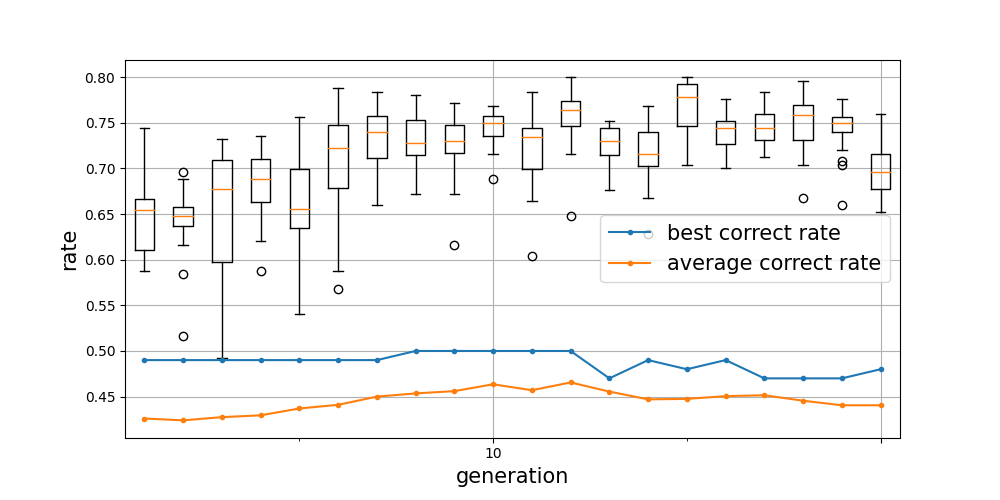
\includegraphics[height=65mm,width=100mm]{graph.png}
		\caption{実験1の結果\label{fig:ex1}}
	\end{center}
\end{figure}
\begin{figure}[h]
	\begin{center}
		\vspace*{-3mm}
		\hspace*{-12mm}
		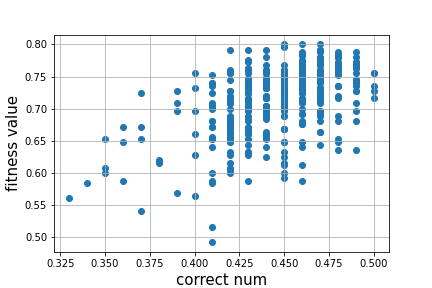
\includegraphics[height=65mm,width=100mm]{img.png}
		\caption{実験1の相関図\label{fig:ex1_1}}
	\end{center}
\end{figure}
また14世代目が適応度の平均が最高であり,その個体を使って再学習したものの精度を表\ref{tb:ex1}示す.閾値はある遺伝子座の採択された遺伝子が全個体に対して占めていた割合に対するものである.
\begin{table}[h]
	\centering
	\caption{GAの設定\label{tb:ex1}}
	\scalebox{1.0}{
		\begin{tabular}{|c|c|c|c|} \hline
			採択数&正答数&閾値&精度\\ \hline
			0&&&0.868\\ \hline\hline
			100&46&なし&0.836\\ \hline
			39&22&0.19&0.862\\ \hline
			19&14&0.2&0.825\\ \hline
		\end{tabular}
	}
\end{table}
増やしたものがラベル付きデータのみを使った時よりも全て低い結果となった.

\subsection{実験2}
実験1を踏まえ,個体評価においてsearch以外のunlabeledが邪魔しているのではと考え,事前学習はFixMatchのまま個体評価に対してFixMatchではなくcross entropy lossのみで学習した.
表\ref{tb:GApara2},\ref{tb:FTXpara2}にパラメータを示す.

\subsubsection{結果}
図\ref{fig:ex2},\ref{fig:ex2_1}に示す.
図\ref{fig:ex2_1}から正答率が増えるほどばらつきがあり,これはデータ数が少ないことに起因しているのではないかと考えられる.
.
\begin{figure}[h]
	\begin{center}
		\vspace*{-3mm}
		\hspace*{-12mm}
		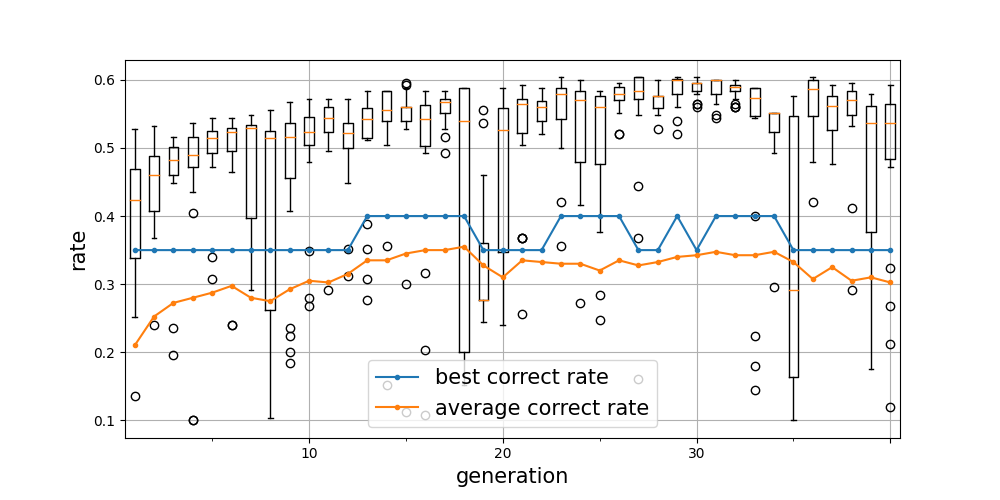
\includegraphics[height=65mm,width=100mm]{graph2.png}
		\caption{実験2の結果\label{fig:ex2}}
	\end{center}
\end{figure}
\begin{figure}[h]
	\begin{center}
		\vspace*{-3mm}
		\hspace*{-12mm}
		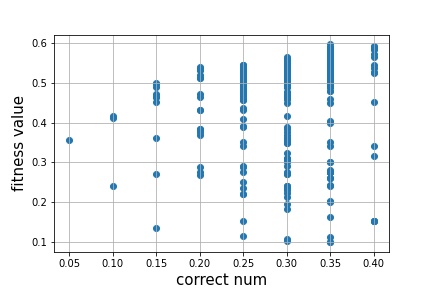
\includegraphics[height=65mm,width=100mm]{img2.png}
		\caption{実験2の相関図\label{fig:ex2_1}}
	\end{center}
\end{figure}


\section{SSLの実験}
GA以外を試す試みとして,FixMatchのlossにVATのlossを入れて実験を行った.
FixMatchのlossに対し0.01の重みを付加してVATのlossを入れた.
\begin{table}[h]
	\centering
	\caption{実験設定\label{tb:FTXpara}}
	\scalebox{1.0}{
		\begin{tabular}{|c|c|c|} \hline
			model&\multicolumn{2}{c|}{WideResNet16-2}\\ \hline\hline
			data set&\multicolumn{2}{c|}{cifar10}\\ \hline
			train &labeled&100\\ \cline{2-3}
			data&unlabeled&49900\\ \hline
			batch size&labeled&32\\ \cline{2-3}
			&unlabeled&$32*7$\\ \hline
			val data&\multicolumn{2}{c|}{10000}\\ \hline\hline
			num\_iterations&\multicolumn{2}{c|}{2**16}\\ \hline
			optimizer&\multicolumn{2}{c|}{SGD(lr=0.1,momntum=0.9)}\\ \hline
		\end{tabular}
	}
\end{table}

表\ref{tb:res}に結果を示す.またこれは2回試行の平均である.
\begin{table}[h]
	\centering
	\caption{結果\label{tb:res}}
	\scalebox{1.0}{
		\begin{tabular}{|c||c|} \hline
			FixMatch&0.849\\ \hline
			FixMatch+VAT&0.857\\ \hline
		\end{tabular}
	}
\end{table}
若干の改善が見れなくもないが検討の余地はあると思われる.

\section{論文の再調査}
GAを用いて半教師あり学習のラベル付きデータを増やす提案はされていたものの,2クラス分類問題に対するものがほとんどであり,cifar10のような画像の分類問題の論文は調べた内にはなかった.\\
\ また,最近の半教師あり学習は自己教師あり学習が組み込まれたものが
精度を出している.手法として以下のものがある.\\
\begin{itemize}
	\item Ensemble AutoEncoder Transform(:EnAET)
	\item Semi-Supervised Self-Supervised Learning(:S4L)
	\item SimCLRv2
	\item CoMatch(MoCo)
\end{itemize}
\ また,vision transformer についても自己教師あり学習により精度の改善があったらしいのでそことも絡められる点でもGAよりも自己教師あり学習を絡めた研究をした方がよいかも知れないと思った.

\section{来週の課題}
\begin{itemize}
	\item 実験設定の改良
	\item 自己教師あり学習の調査
\end{itemize}


\begin{table}[h]
	\centering
	\caption{GAの設定\label{tb:GApara}}
	\scalebox{1.0}{
		\begin{tabular}{|c||c|} \hline
			個体数&20\\ \hline
			世代数&20\\ \hline
			交叉率&1.0\\ \hline
			突然変異率&0.02\\ \hline\hline
			labeled&250枚\\ \hline
			search&100枚\\ \hline
		\end{tabular}
	}
\end{table}

\begin{table}[h]
	\centering
	\caption{FixMatchの設定\label{tb:FTXpara}}
	\scalebox{1.0}{
		\begin{tabular}{|c|c|c|} \hline
			model&\multicolumn{2}{c|}{WideResNet16-2}\\ \hline\hline
			data set&\multicolumn{2}{c|}{cifar10}\\ \hline
			batch size&labeled&32\\ \cline{2-3}
			&unlabeled&$32*7$\\ \hline
			optimizer&\multicolumn{2}{c|}{SGD(lr=0.1,momntum=0.9)}\\ \hline
			loss&\multicolumn{2}{c|}{cross\_entropy\_loss}\\ \hline\hline
			\multicolumn{3}{|c|}{事前学習}\\ \hline
			train &labeled&100\\ \cline{2-3}
			&unlabeled&49650\\ \hline			
			val data&\multicolumn{2}{c|}{150}\\ \hline
			num\_iterations&\multicolumn{2}{c|}{2**15}\\ \hline\hline
			\multicolumn{3}{|c|}{GAの評価}\\ \hline
			train &searchのみ&100\\ \cline{2-3}
			&unlabeled&49650\\ \hline
			val data&\multicolumn{2}{c|}{250}\\ \hline
			num\_iterations&\multicolumn{2}{c|}{5000}\\ \hline\hline
			\multicolumn{3}{|c|}{得られた個体の評価}\\ \hline
			train &labeled+search&250+?\\ \cline{2-3}
			&unlabeled&49650\\ \hline	
			val data&\multicolumn{2}{c|}{10000}\\ \hline
			num\_iterations&\multicolumn{2}{c|}{2**16}\\ \hline
		\end{tabular}
	}
\end{table}

\begin{table}[h]
	\centering
	\caption{GAの設定\label{tb:GApara2}}
	\scalebox{1.0}{
		\begin{tabular}{|c||c|} \hline
			個体数&20\\ \hline
			世代数&40\\ \hline
			交叉率&1.0\\ \hline
			突然変異率&0.02\\ \hline\hline
			labeled&100枚\\ \hline
			search&20枚\\ \hline
		\end{tabular}
	}
\end{table}

\begin{table}[h]
	\centering
	\caption{FixMatchの設定\label{tb:FTXpara2}}
	\scalebox{1.0}{
		\begin{tabular}{|c|c|c|} \hline
			model&\multicolumn{2}{c|}{WideResNet16-2}\\ \hline\hline
			data set&\multicolumn{2}{c|}{cifar10}\\ \hline
			batch size&labeled&32\\ \cline{2-3}
			&unlabeled&$32*7$\\ \hline
			optimizer&\multicolumn{2}{c|}{SGD(lr=0.1,momntum=0.9)}\\ \hline
			loss&\multicolumn{2}{c|}{cross\_entropy\_loss}\\ \hline\hline
			\multicolumn{3}{|c|}{事前学習}\\ \hline
			train &labeled&10\\ \cline{2-3}
			&unlabeled&49880\\ \hline			
			val data&\multicolumn{2}{c|}{90}\\ \hline
			num\_iterations&\multicolumn{2}{c|}{2**15}\\ \hline\hline
			\multicolumn{3}{|c|}{GAの評価}\\ \hline
			train &searchのみ&20\\ \cline{2-3}
			&unlabeled&49880\\ \hline
			val data&\multicolumn{2}{c|}{250}\\ \hline
			num\_iterations&\multicolumn{2}{c|}{5000}\\ \hline
		\end{tabular}
	}
\end{table}



\end{document}


